\section{Runtime comparison with the Cangjie standard library}
\label{sec:benchmarks}

The generated implementations were benchmarked against the standard
linked list, array, array list, and hash map, specialized at \texttt{Int64},
on 30 September 2026.
The compiler and the standard library were those of Cangjie 1.0.5 (cjnative),
with optimization \texttt{-O2}, targeting \texttt{aarch64-apple-darwin}.
The machine was an Apple M4 Mac mini, with ten cores (four performance and
six efficiency), 16 GB RAM, and macOS 26.6.2.  These measurements compare
the actual printed programs with the SDK's standard types; they do not
establish the performance-parity claim for all CJR programs.

\subsection{Method and comparable workloads}

Each of the four unchanged generated source files was compiled with a
Cangjie benchmark test containing both implementations.  The executable
ran in three independent processes, sequentially, with seven samples of
each implementation at each size in each process.  The 36 workload/size
points therefore produced 1,512 timed samples.  Both implementations were
warmed up, and their batch sizes were calibrated independently toward
20 milliseconds.  Allocating workloads were capped at $262144/n$
repetitions; other workloads at 65,536.  The shortest observed batch was
838 microseconds.  The order of the two implementations alternated between
trials.  There was no core pinning, forced garbage collection, or subtraction
of an empty-loop timing.

The timer was \texttt{std.time.MonoTime.now()}.  Compilation, test-framework
setup, steady-state data preparation, printing, and checksum checks were
excluded from the timed intervals.  Loop and callback overheads were
included.  Each measured batch returned an observable checksum which was
checked after timing; all twelve process-level benchmark suites passed.
Map setup checked every key and value, and array-list rotation checked that
the final sequence and size were restored.

\paragraph{Lists.} A traversal sums the contents via CJR's
\texttt{head}/\texttt{tail}, or the standard list's
\texttt{firstNode}/\texttt{next}.  Prepend-and-scan builds the same sequence
and traverses it, including allocation.  Sizes are 256, 4,096, and 16,384;
the unit is time per visited node, or per inserted-and-visited item.
The generated list is singly linked, whereas the standard list is doubly
linked and maintains collection membership.  This is a comparison of
common operations, not of identical representations or guarantees.

\paragraph{Arrays.} The indexed read visits every initialized cell in the
order $(17i) \bmod n$.  A write-and-read batch performs $n$ writes and then
$n$ reads, dividing its time by $2n$.  The sizes are 256, 4,096, and 65,536.
Every raw CJR cell is explicitly initialized before its first read; array
constructors are excluded.  CJR accesses raw pointers without bounds
checks, whereas the standard array is indexed through its public API.

\paragraph{Array lists.} Indexed read uses the same permutation.
Append-and-scan starts at the default constructor, appends $n$ values with
natural capacity growth, then reads them all; its unit is one
inserted-and-visited item.  Both use $n=256,4096,16384$.
Front rotation removes index zero and appends the removed value, $n$ times,
restoring the sequence; its unit is one remove/append pair and its sizes
are 256, 1,024, and 4,096.  Setup is excluded for reads and rotations.

\paragraph{Hash maps.} Insert-and-scan includes default construction,
growth, insertion of keys $0,\ldots,n-1$ with values $3i+1$, and reading
every key.  Hit and miss batches query $0,\ldots,n-1$ and
$n,\ldots,2n-1$ respectively.  A large-key hit batch uses
$1000000,\ldots,1000000+n-1$.  These workloads use sizes 256, 4,096, and
16,384.  The collision workload uses keys $i(2n)$, at sizes 256, 1,024, and
4,096.  They all start in bucket zero at the CJR map's final capacity $2n$;
the standard map receives exactly the same keys, using its own bucket
policy.  Successful reads check presence on both sides.  Lookup setup is
excluded.  Insert-and-scan time is per inserted-and-read item; other map
time is per query.

\subsection{Measured results}

Figure~\ref{fig:benchmark-overview} shows the median paired time ratio at
the largest tested size of each workload.  A ratio below one means the
generated code ran faster.  There are 21 paired samples per point; the
whiskers show their interquartile range, not a confidence interval.
The following table also gives the individual median times.  Different
rows have the workload units defined above, so their absolute values
should not be compared as if each row timed the same operation.

\begin{center}
\small
% Generated by benchmark/plot.py from benchmark/results/raw.csv and summary.json.
\begin{tabular}{@{}lrrrr@{}}
\hline
Workload & $n$ & CJR (ns) & Std (ns) & Ratio \\
\hline
Linked lists: Traverse & 16,384 & 1.78 & 2.21 & 0.80 \\
Linked lists: Prepend + scan & 16,384 & 4.31 & 14.84 & 0.29 \\
Arrays: Indexed read & 65,536 & 0.98 & 0.81 & 1.22 \\
Arrays: Write + read passes & 65,536 & 0.92 & 0.57 & 1.63 \\
Array lists: Indexed read & 16,384 & 1.21 & 0.86 & 1.40 \\
Array lists: Append + scan & 16,384 & 3.57 & 4.25 & 0.84 \\
Array lists: Front removal + append & 4,096 & 5016.36 & 318.01 & 15.70 \\
Hash maps: Insert + scan & 16,384 & 25.47 & 18.43 & 1.38 \\
Hash maps: Lookup hit & 16,384 & 5.85 & 2.39 & 2.46 \\
Hash maps: Lookup miss & 16,384 & 4.09 & 1.66 & 2.45 \\
Hash maps: Large-key hit & 16,384 & 17.84 & 2.39 & 7.40 \\
Hash maps: Colliding hit & 4,096 & 19445.07 & 1006.32 & 19.30 \\
\hline
\end{tabular}

\end{center}

\begin{figure}[!htbp]
\centering
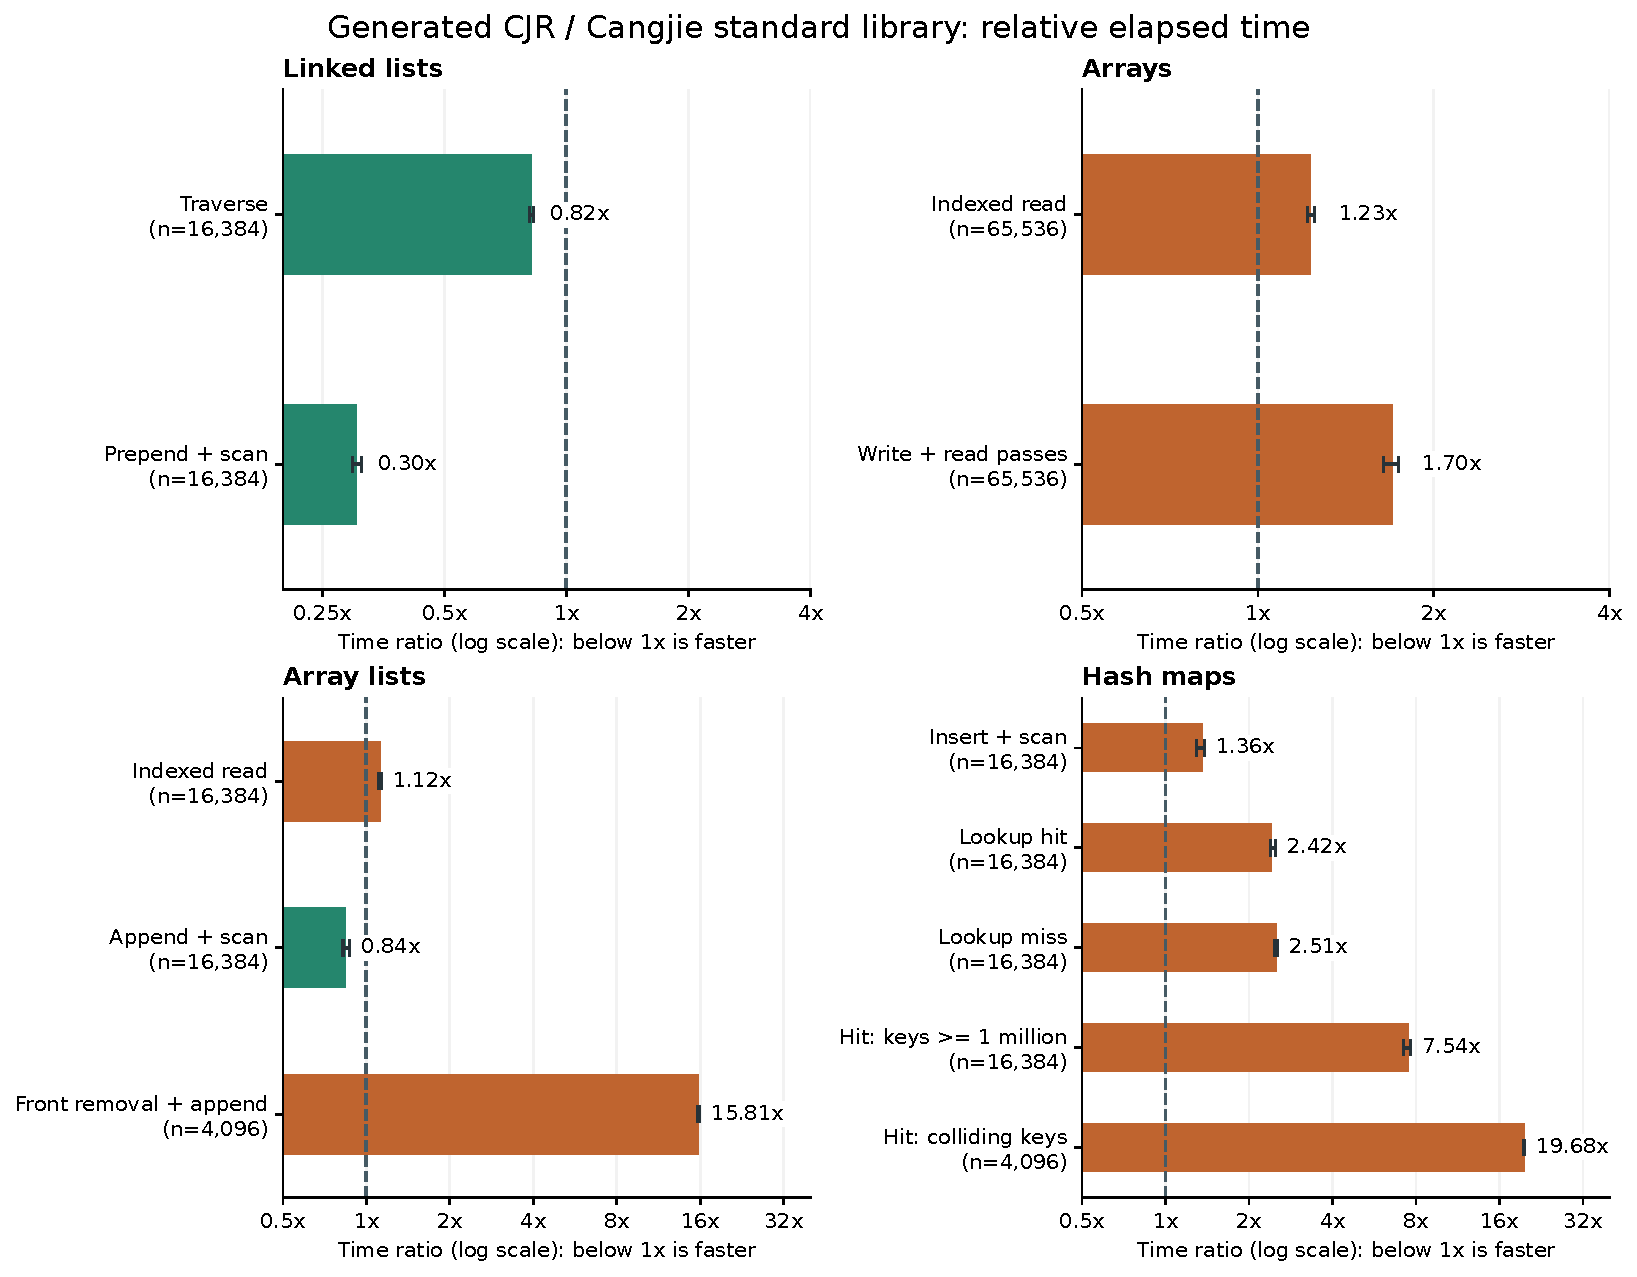
\includegraphics[width=\textwidth]{paper/figures/benchmark-overview.pdf}
\caption{Relative elapsed time of generated CJR and standard-library
workloads at their largest tested sizes.  The dashed line is equal time;
bars and error whiskers are the median and interquartile range of paired
CJR/standard ratios.  List build/scan, array-list build/scan, and map
build/scan include construction and growth; the other setups are excluded.}
\label{fig:benchmark-overview}
\end{figure}

\paragraph{Lists and arrays.} Prepend-and-scan on the smaller CJR list
representation takes about 0.30 times the standard list time, and traversal
about 0.82 times.  Those results reflect the different list representations,
as well as optimization and runtime behavior.  The generated arrays are
not faster in these tests: indexed read takes 1.23 times the standard-array
time, and the write/read workload 1.70 times.  The lack of raw-pointer bounds
checks therefore does not imply a measured speed advantage for these loops.

\paragraph{Array lists.} Append-and-scan takes about 0.84 times the standard
time, while indexed read takes 1.12 times.  Front rotation is much more
expensive: about 15.81 times the standard time at $n=4096$.  The generated
\texttt{remove} explicitly reads and writes every shifted word.  These
measurements establish the observed cost difference, without an assembly
analysis identifying all compiler and library contributions to it.

\paragraph{Hash maps.} Ordinary successful lookup takes about 2.42 times
the standard time, misses 2.51 times, and insert-and-scan 1.36 times at
$n=16384$.  The key pattern can cause a much greater slowdown.  The
large-key workload at $n=256$ has median times of approximately 670.5 ns
and 2.4 ns per query (roughly 280 times slower for CJR).  At $n=16384$,
the paired ratio is still 7.54.  Colliding keys at $n=4096$ take about
19.68 times the standard time.  Both maps slow down on this collision
workload; the generated map does not have uniform lookup performance.

\begin{figure}[!htbp]
\centering
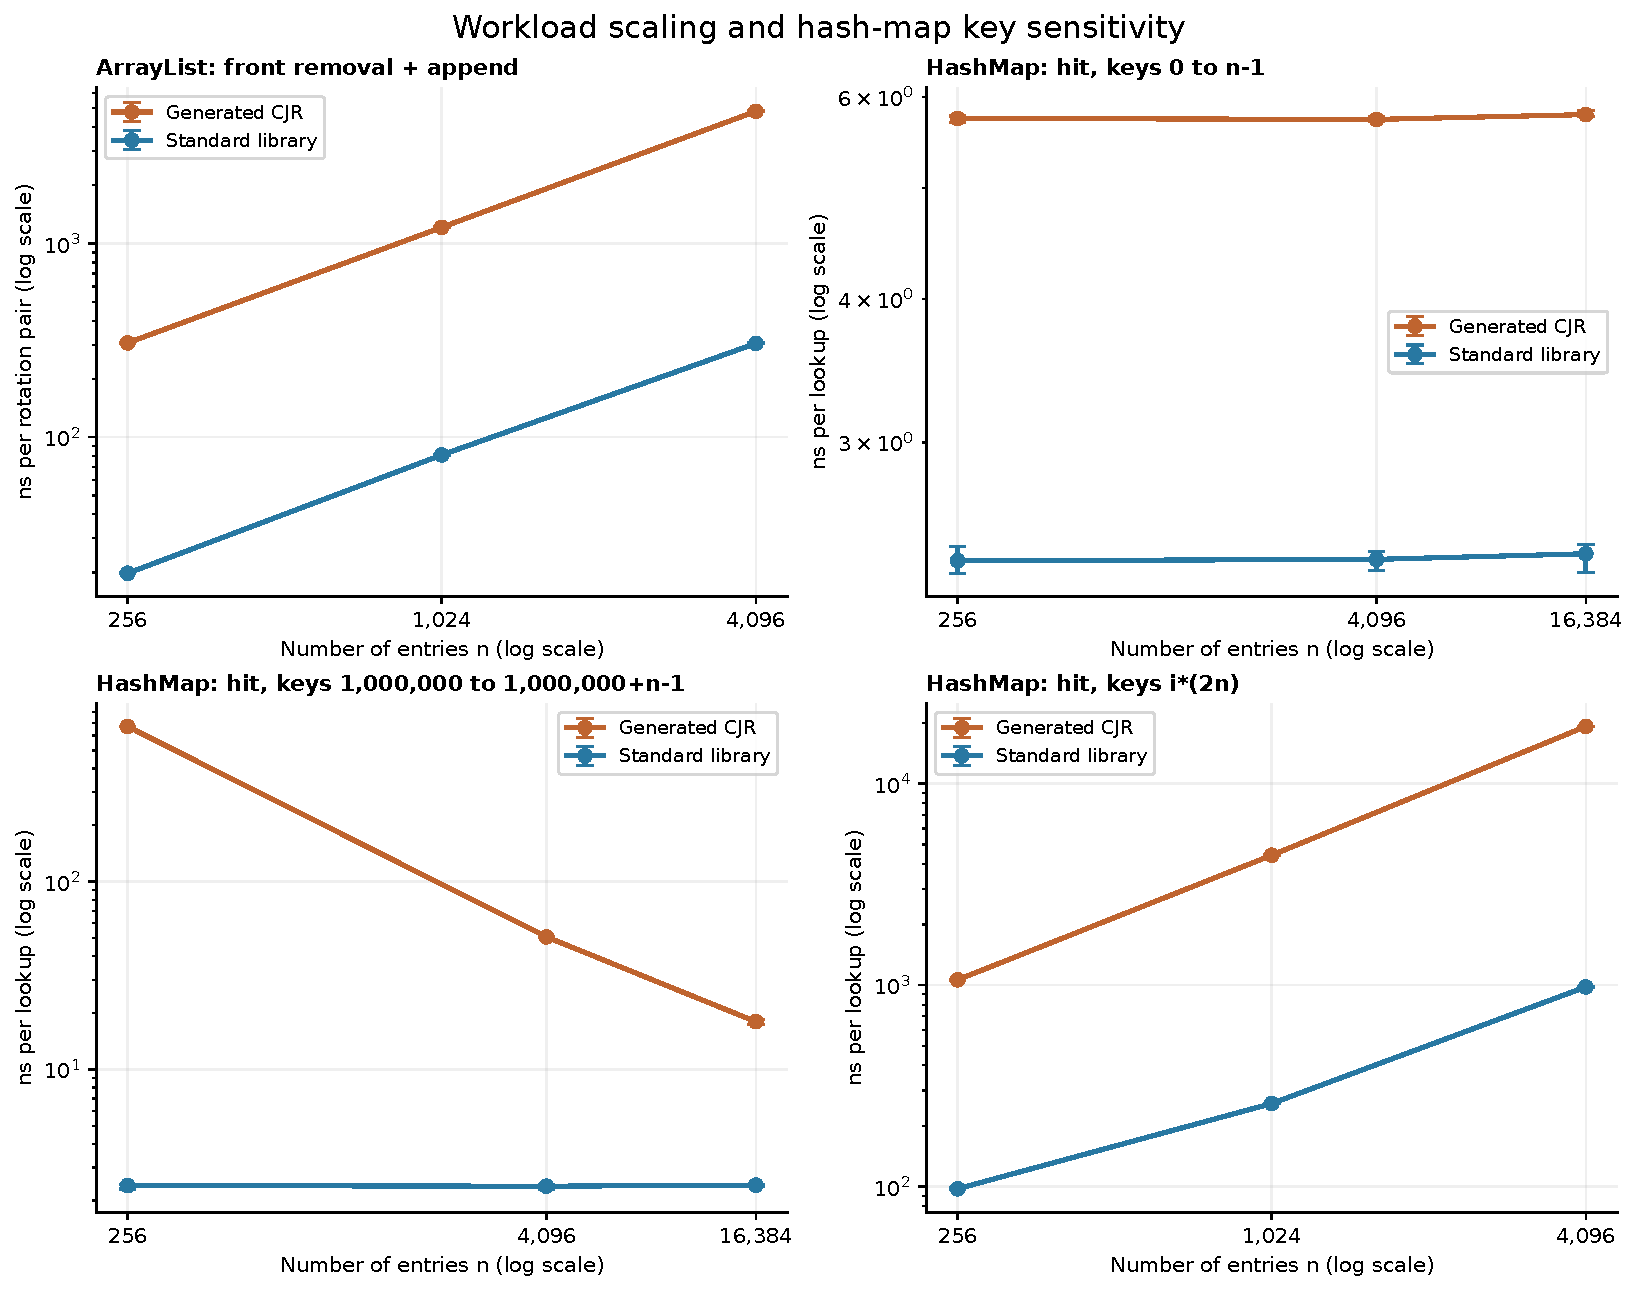
\includegraphics[width=\textwidth]{paper/figures/benchmark-scaling.pdf}
\caption{Scaling of front rotation and hash-map queries.  Both axes use
logarithmic scales.  Lines show individual median times, with interquartile
error whiskers.  In the large-key case, the CJR time falls as capacity grows,
because remainder normalization needs fewer subtractions.  Colliding keys
show increasing query costs for both implementations.}
\label{fig:benchmark-scaling}
\end{figure}

\subsection{Interpretation, limitations, and reproduction}

The large-key behavior has a concrete source-level explanation: CJR's
\texttt{residue} routine repeatedly subtracts the capacity.  A small map
needs many such steps for keys near one million; a larger map needs fewer.
The collision workload also combines a long probe with a costly remainder
calculation.  These are valid keys and are materially different from the
sequential-key test.  The measurements do not justify treating all hash-map
keys as equally cheap or extrapolating to the extremes of \texttt{Int64}.

The generated resizable buffers never free their old \texttt{malloc}
blocks.  The harness does not repair that behavior or free buffers; batch
limits and process exits bound the experiment's allocation pressure.
Standard arrays and collections use the managed runtime instead.  This
comparison includes their natural allocation costs, but it is not a
measurement of sustained memory consumption or the cost of reclamation
that a production raw-memory implementation would need.

Similarly, raw array construction is not equivalent to the standard array's
initialized construction.  Explicitly writing cells before reads avoids
using uninitialized contents in the array timing.  The generated map still
relies on zero-valued fresh tags: its checks passed on this runtime, but
the benchmark does not establish or fix the allocation assumption discussed
in Appendix~\ref{sec:limitations}.  The tests use valid indexes, bounded
values, a warm working set, and single-threaded code on an unpinned desktop
process.  They support workload-specific comparisons on this machine,
not a general correctness, complexity, or performance theorem.

The reproducible harness is in \texttt{benchmark/}.  The unchanged source
hashes, compiler configuration, every timed sample, and summary statistics
are recorded in \path{benchmark/results/metadata.json},
\texttt{raw.csv}, and \texttt{summary.json}.  The figures and table are
generated from that data by \path{benchmark/plot.py}.  Re-run
\texttt{python3 benchmark/run.py} with the matching SDK and linker SDK
paths, followed by \texttt{python3 benchmark/plot.py} (Matplotlib is
required).  \texttt{benchmark/README.md} explains the exact build command,
units, warmups, repetitions, and the existing macOS linker-stub workaround.
